% !TEX root = ../../main_without_quantization.tex
\section{The Genetic Search Algorithm}
\label{chap:ga}

The search stage receives the fixed mask representation, the compute budget, and the ranking metric defined in the preceding sections. Its role is to select one feasible architecture for recovery. The search cannot use gradients with respect to the binary masks, and exhaustive enumeration is infeasible. The procedure therefore uses an evolutionary search that keeps multiple feasible candidates alive, evaluates only a bounded number of masks, and returns the best mask found under the surrogate ranking.

The detailed presentation is written for encoder pruning. The decoder searches follow the same overall procedure, and decoder-specific changes are stated where they are needed.

\subsection{The Level Database}
\label{ga:level_db}

The three decoder searches, namely quantization, low-rank factorisation, and rank-based recovery, rely on a \emph{level database} built once before the search begins. The quantization database stores one compressed matrix and its size cost for each available bit-width. The low-rank database stores one factorised matrix and its parameter cost for each retained-rank level. The recovery database stores the residual-rank additions and their costs. A candidate is then assembled by selecting entries from the relevant database, so evaluation only requires a forward pass and feasibility can be checked from the stored costs. This follows the level-database idea used in EvoPress \citep{evopress2024} and the sparsity-level database of DarwinLM \citep{darwinlm2025}.

\begin{figure}[htbp]
\centering
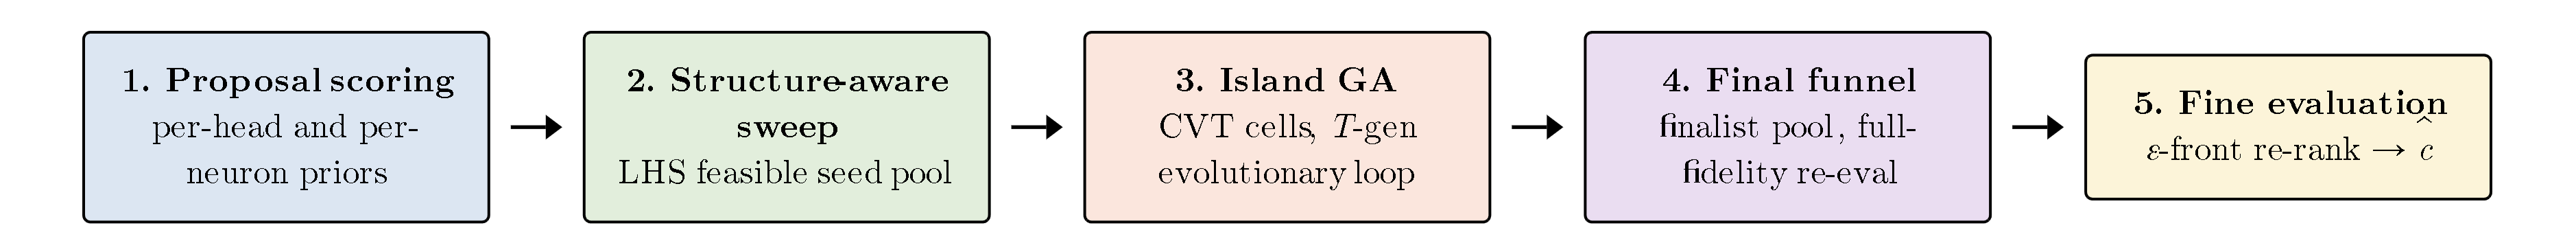
\includegraphics[width=0.95\linewidth]{figures/five-phase-genetic-search.png}
\caption{Five-phase overview of the genetic search. Phase 1 computes proposal scores from the teacher on the fixed evaluation subset. Phase 2 builds a feasible seed pool by a structure-aware sweep. Phase 3 runs the island GA: a Centroidal Voronoi Tessellation (CVT) partition of $\mathcal{X}_\budget$ \citep[see Appendix~\ref{sec:appendix_cvt}]{du1999centroidal} and a $T$-generation evolutionary loop with archive updates. Phase 4 pools finalists and re-evaluates them at full fidelity. Phase 5 selects $\widehat{\cand}$ from the pooled finalists.}
\label{fig:ga_five_phase}
\end{figure}

\subsection{Search Interface and Feasibility Objective}
\label{ga:inputs}

The previous sections define the pieces of the pruning problem in isolation. Of course, they need to be assembled into a concrete selection process, this is where the search stage comes in. It uses the representation, the budget model, and the ranking metric as fixed inputs to identify one feasible architecture for recovery.

Figure~\ref{fig:search-inputs} summarizes the interface of the search stage. The search receives three fixed objects from the previous sections: the candidate representation, the target compute budget, and the surrogate metric. It returns a single mask $\hat{c}$ that satisfies the structural and computational constraints while minimizing the surrogate distance among the candidates explored by the search procedure.

\begin{figure}[htbp]
    \centering
    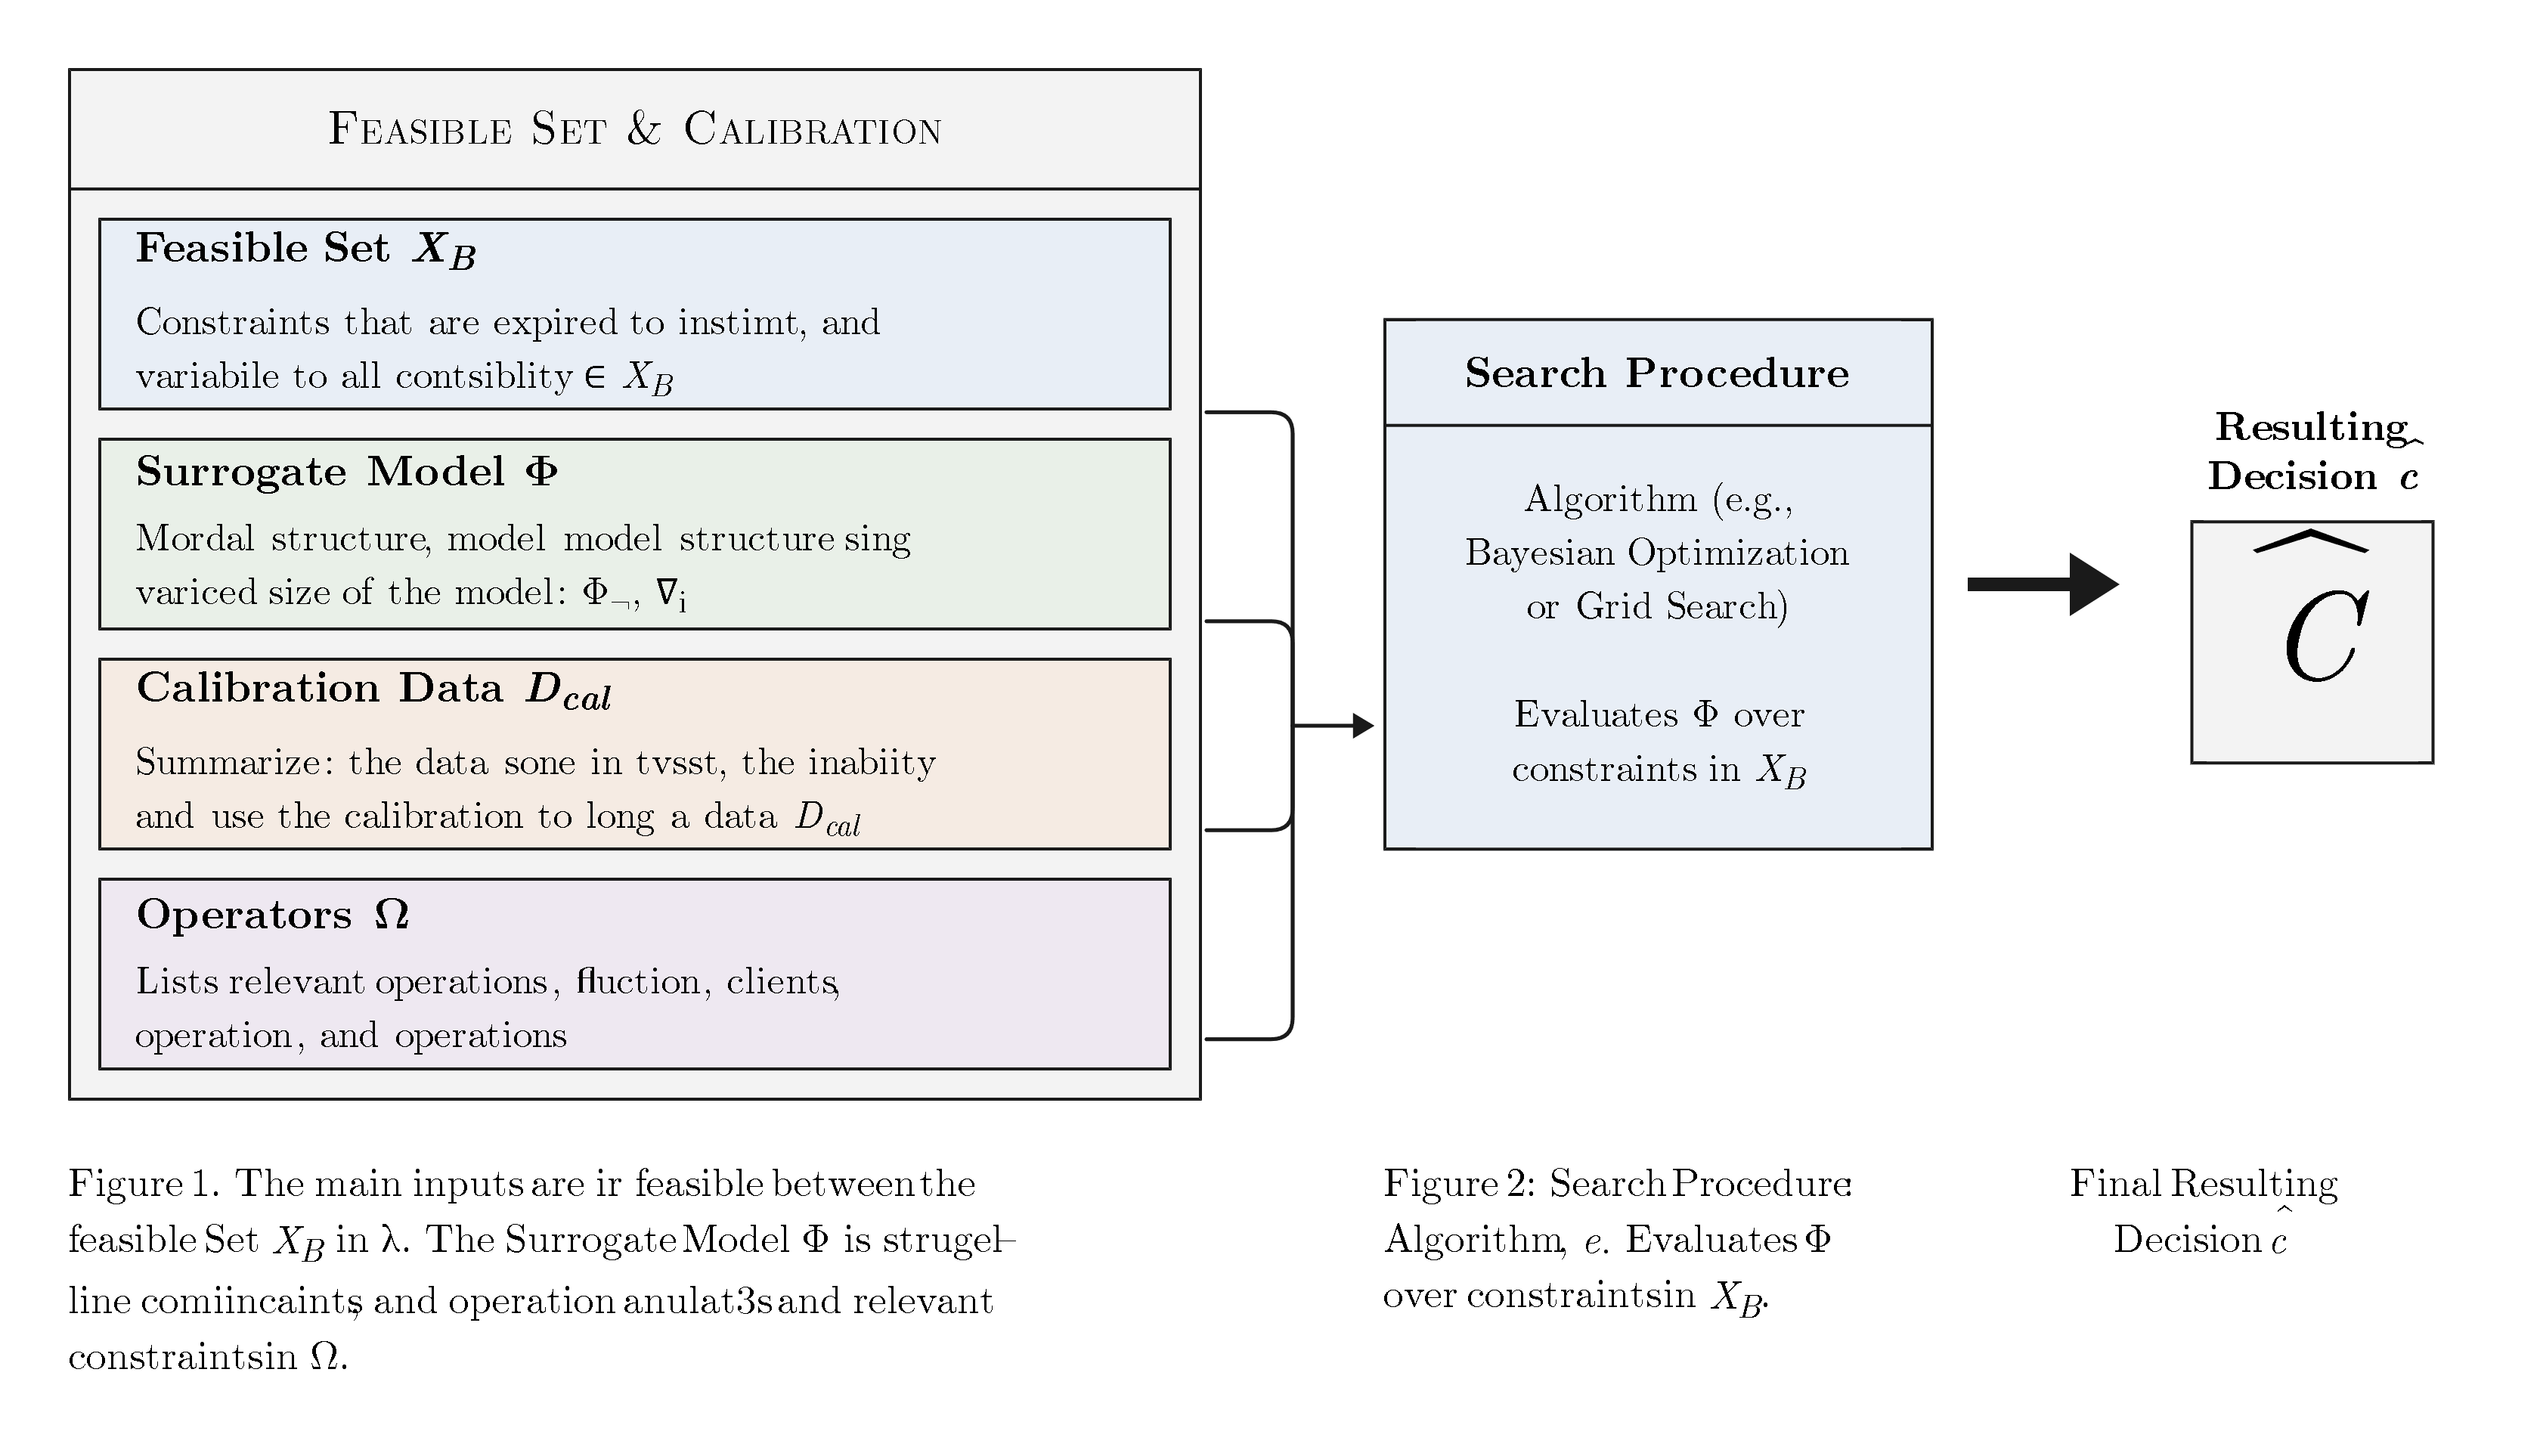
\includegraphics[width=0.7\linewidth]{figures/ga_overview_1.png}
    \caption{Inputs and output of the search stage. The candidate representation, compute budget, and surrogate metric are fixed before search. The search procedure explores feasible candidates and returns one selected mask $\hat{c}$ for recovery.}
    \label{fig:search-inputs}
\end{figure}

For encoder pruning, feasibility is defined by two constraints: the operation cost must lie inside the target budget band, and the active depth must remain above a minimum value. The cost band admits the compact formulation below. A candidate
\[
c = \left(M^{H}, \{n_l\}_{l=1}^{L}\right)
\]
specifies a head mask and a per-layer neuron count, as defined in Section~\ref{chap:mask}. Its operation cost $\operatorname{MAC}(c)$ follows from these choices through the cost model of Section~\ref{chap:cost}. The cost model restricts admissible candidates to the feasibility band
\[
\mathcal{X}_{B}
=
\left\{
c :
(1-\varepsilon)B
\leq
\operatorname{MAC}(c)
\leq
(1+\varepsilon)B
\right\}.
\]

Inside this band, the surrogate distance $\Phi$ of Section~\ref{chap:metric} ranks candidates against the teacher on the fixed metric subset. The active-depth floor
\[
N_a(c) \geq L_{\min}
\]
keeps at least $L_{\min}$ layers active. Equivalently, the complete feasible set can be written as
\[
\mathcal{F}_{B}
=
\left\{
c \in \mathcal{X}_{B}
:
N_a(c) \geq L_{\min}
\right\}.
\]

The search returns the mask that minimises the surrogate distance over this restricted feasible set:
\[
\hat{c}
\in
\arg\min_{c \in \mathcal{F}_{B}}
\Phi(c).
\]

The objective above defines the mask selected by our method. To approximate this objective under the finite evaluation budget, we organize the search as a structured genetic procedure over the feasible band $\mathcal{F}_{B}$. The procedure is designed to maintain diversity across distinct regions of the budget-constrained space, enforce feasibility after candidate modifications, and reserve higher-fidelity evaluation for the most competitive masks. The next subsection details this procedure and describes how it produces the final selected mask $\hat{c}$.

\subsection{The Five-Phase Genetic Procedure}
\label{ga:overview}

The combinatorial size of $\mathcal{X}_\budget$ and the bounded evaluation budget shape the five-phase structure of the procedure. Phases~1 and~2 prepare the search state with per-head and per-neuron proposal scores and a feasible seed pool. Phase~3 runs the iterated evolutionary loop over regional populations, accumulating best candidates into three global archives. Phases~4 and~5 collapse the search state: a final funnel re-evaluates pooled finalists at full fidelity, and a fine-evaluation step selects $\widehat{\cand}$ under an $\epsilon$-front tie-break.

\subsubsection{Phase 1: Proposal Scoring}
\label{ga:phase_proposals}

Before any candidate is constructed, the procedure computes per-head and per-neuron Fisher-style local sensitivities of the teacher on the calibration set, denoted $s_H[\ell,h]$ and $s_N[\ell,n]$. The per-layer aggregate
\[
\mathrm{imp}(\ell) \;=\; \sum_h s_H[\ell,h] \;+\; \sum_n s_N[\ell,n]
\]
is a layer importance prior. The proposal scores drive the mechanics of the encoder search. Since the search edits very fine-grained units, heads and neurons are sampled stochastically rather than by always deleting the lowest-scoring unit. The sampling probability is importance-weighted, so low-importance units still have a smaller chance of being selected, while the search keeps enough randomness to explore alternative masks. The same scores are also used when projecting a candidate back into the feasible band after an edit.

For the decoder searches, the architecture space is much larger and this head-and-neuron proposal stage is not used. Quantization, low-rank factorisation, and rank-based recovery instead use the prebuilt level databases of Section~\ref{ga:level_db}. Layer drop is the exception: it does not require a level database, because a candidate only selects which attention and feed-forward sub-blocks are kept or skipped.

\subsubsection{Phase 2: Structure-Aware Sweep}
\label{ga:phase_sweep}

The initial seed pool for encoder pruning is built by a Latin hypercube sweep \citep{mckay1979comparison} over three axes: the active-layer count $\nactive$, the fraction $\phi_H$ of the operation budget spent on attention heads, and a subset mode that decides how the active layers are drawn from $\mathrm{imp}(\ell)$. Latin hypercube sampling is used here as a stratified design: each axis is divided into intervals, and the sweep draws combinations that cover the range of each axis without requiring a full grid. For each sampled cell, a candidate is constructed with the chosen $\nactive$ active layers and the chosen split of MAC between heads and neurons, then projected into $\mathcal{X}_\budget$. The sweep returns a pool of feasible candidates spread across coarse macro descriptors.

For the decoder searches, the seed pool is built directly from feasible level vectors, since the genomes are layer-wise bit, rank, recovery, or drop decisions rather than head-and-neuron masks. These feasible decoder candidates are then mapped to the same kind of low-dimensional descriptor space used for the CVT partition. In both cases, the seed pool serves two roles in Phase~3: it initializes the regional populations and provides the sample from which $\mathcal{X}_\budget$ is partitioned into regions of similar candidates by a \emph{Centroidal Voronoi Tessellation} (CVT) \citep[see Appendix~\ref{sec:appendix_cvt}]{du1999centroidal}.

\subsubsection{Phase 3: Island GA}
\label{ga:phase_island}
\label{chap:islands}
\label{chap:operators}
\label{ga:projection}

In the third phase, multiple populations explore the feasible band $\mathcal{X}_\budget$ while each is rooted in a separate portion of the band. Thus local refinement and wider exploration may occur in parallel. Many feasible masks are close to each other: that is, they are only separated by minor budget-preserving edits such as moving active heads, relocating blocks of neurons in or between layers, or altering head--neuron balance such that the MAC cost remains almost the same. Such edits are consistent with preserving the candidate structure and are thus well-suited to local refinement.

Other masks which also fit within the MAC budget, might be constructed with capacity in different locations within the layers. For example, one mask could leave capacity mostly with early layers, one might favor later layers, or it might select entirely different layers to remain active. They correspond to points which may not be small perturbations of the same candidate but are instead independent exploration targets.

\begin{figure}[H]
\centering
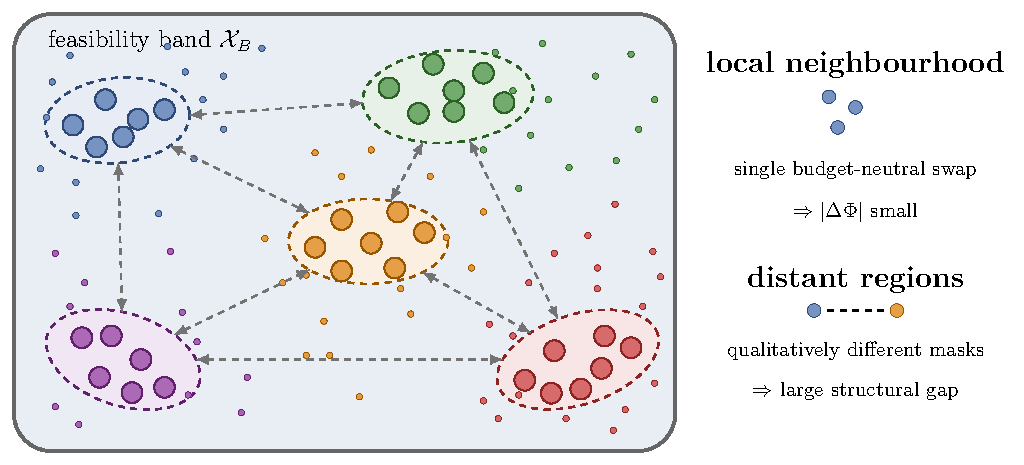
\includegraphics[width=0.6\linewidth]{figures/ga_overview_2.pdf}
\caption{The feasibility band $\mathcal{X}_\budget$ as a populated space. Feasible candidates form clusters of architecturally similar masks; clusters in different regions of the band differ qualitatively.}
\label{fig:ga_overview_2}
\end{figure}

The third phase encodes this two-scale structure through a \emph{Centroidal Voronoi Tessellation} (CVT) of the feasible candidate space $\mathcal{X}_\budget$ \citep[see Appendix~\ref{sec:appendix_cvt}]{du1999centroidal}. Each candidate is first mapped to a six-dimensional descriptor $z(\cand)\in[0,1]^6$, and $k$-means is applied to the descriptor vectors from the seed pool. The descriptor is family-specific: encoder pruning uses head, neuron, active-depth, entropy, and depth-centre statistics, while the decoder searches use descriptors built from their level vectors. The full descriptor definitions are reported in Appendix~\ref{sec:appendix_descriptors}. Each Voronoi cell defines an island's basin; a population of size $P$ is seeded inside each basin from the sweep pool of Phase~\ref{ga:phase_sweep}, projected into the basin's bounds. Local refinement is then carried out inside each island, while the partition itself enforces coverage across regions.

\begin{figure}[htbp]
\centering
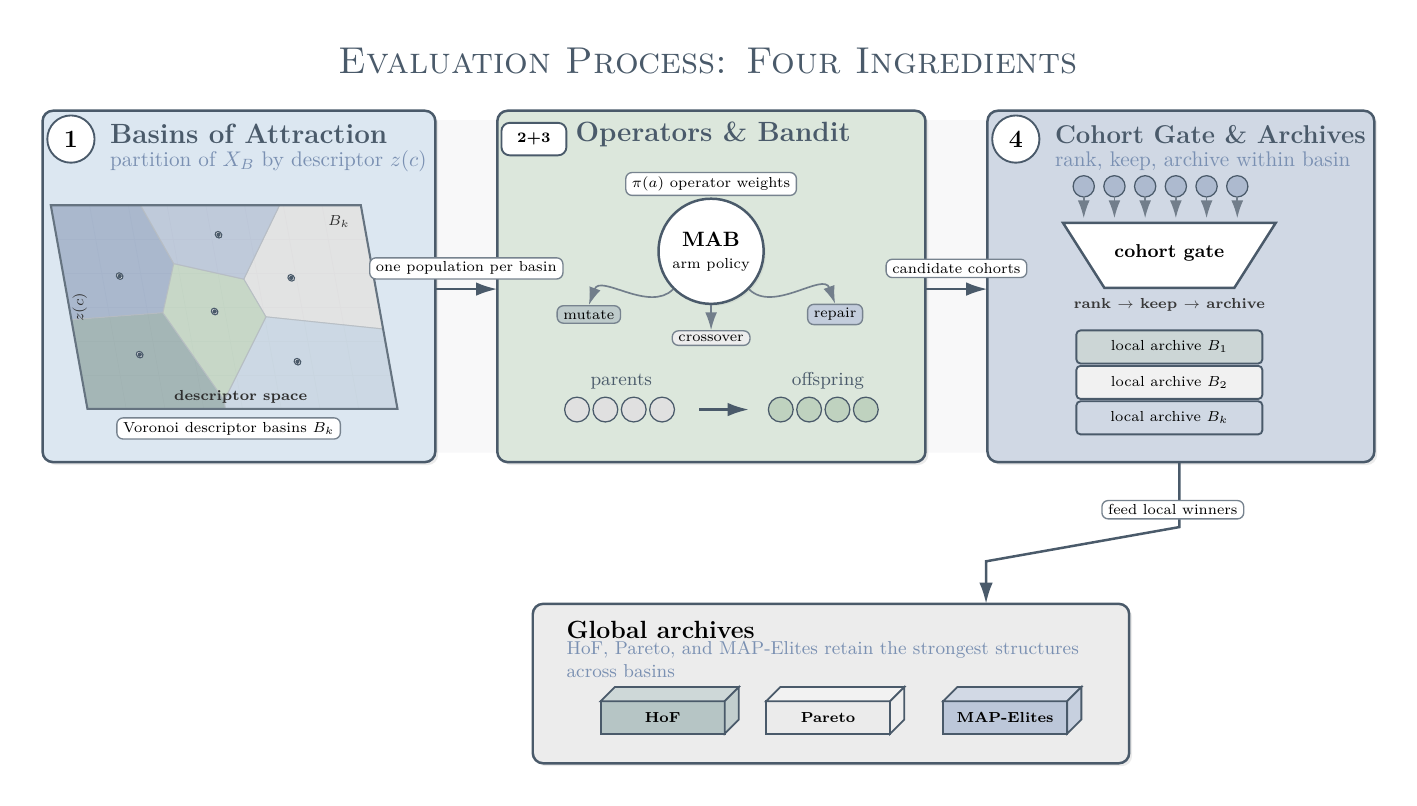
\includegraphics[width=1.0\linewidth]{figures/ga_overview_3.png}
\caption{The four pieces of machinery inside the generational loop. Regions maintain separate populations, operators produce feasible offspring after repair, bandits adapt operator probabilities, and selection feeds both the next population and the archives.}
\label{fig:ga_overview_3}
\end{figure}

Within this partition, the loop runs for $T$ generations (Figure~\ref{fig:ga_overview_4}). In each generation, per island: parents are chosen by a tournament rule whose score combines a fitness-shared rank (each rank divided by a structural-crowding count) with a novelty bonus equal to the minimum mask-distance to already-selected parents; offspring are produced by crossover and mutation operators drawn from an EXP3-IX bandit local to the island (Appendix~\ref{sec:appendix_exp3ix}); each offspring is projected back into the basin to enforce the budget band and the basin bounds; offspring are evaluated by $\score$ at cheap number of calibration tokens, with a scheduled subset re-evaluated at higher number of tokens; and the union of incumbents and offspring is ranked by the two-step cohort rule of Section~\ref{metric:cohort}. Survivors form the next-generation population. The best-scoring candidates of the cohort are inserted into three global archives: a Hall of Fame keyed by exact mask signature, a Pareto front on $(\score, \macop)$, and a MAP-Elites grid keyed by $(\nactive, \phi_H)$.

\subsubsection{Phase 4: Final Funnel}
\label{ga:phase_funnel}

After $T$ generations, the procedure assembles a finalist pool from four sources: the global best candidate observed across the run, the top candidates of each island's final population, samples from the three archives (Hall of Fame, Pareto front, MAP-Elites), and the global best running incumbent (Figure~\ref{fig:ga_overview_4}). The pool is deduplicated by exact mask signature. Each finalist is then re-evaluated on the full-fidelity calibration pack with $R$ independent resamples averaged into a single score.

\subsubsection{Phase 5: Fine Evaluation}
\label{ga:phase_fine}

The averaged finalist scores define an $\epsilon$-front: the candidates whose resampled $\score$ lies within $\epsilon$ of the lowest score in the finalist pool. The $\epsilon$-front is sorted lexicographically by $(\score, -\macop)$, so among candidates within calibration noise of one another the procedure prefers the one that uses more of the allowed compute. The first element of the sort is returned as $\widehat{\cand}$ (Figure~\ref{fig:ga_overview_4}).

\begin{figure}[htbp]
\centering
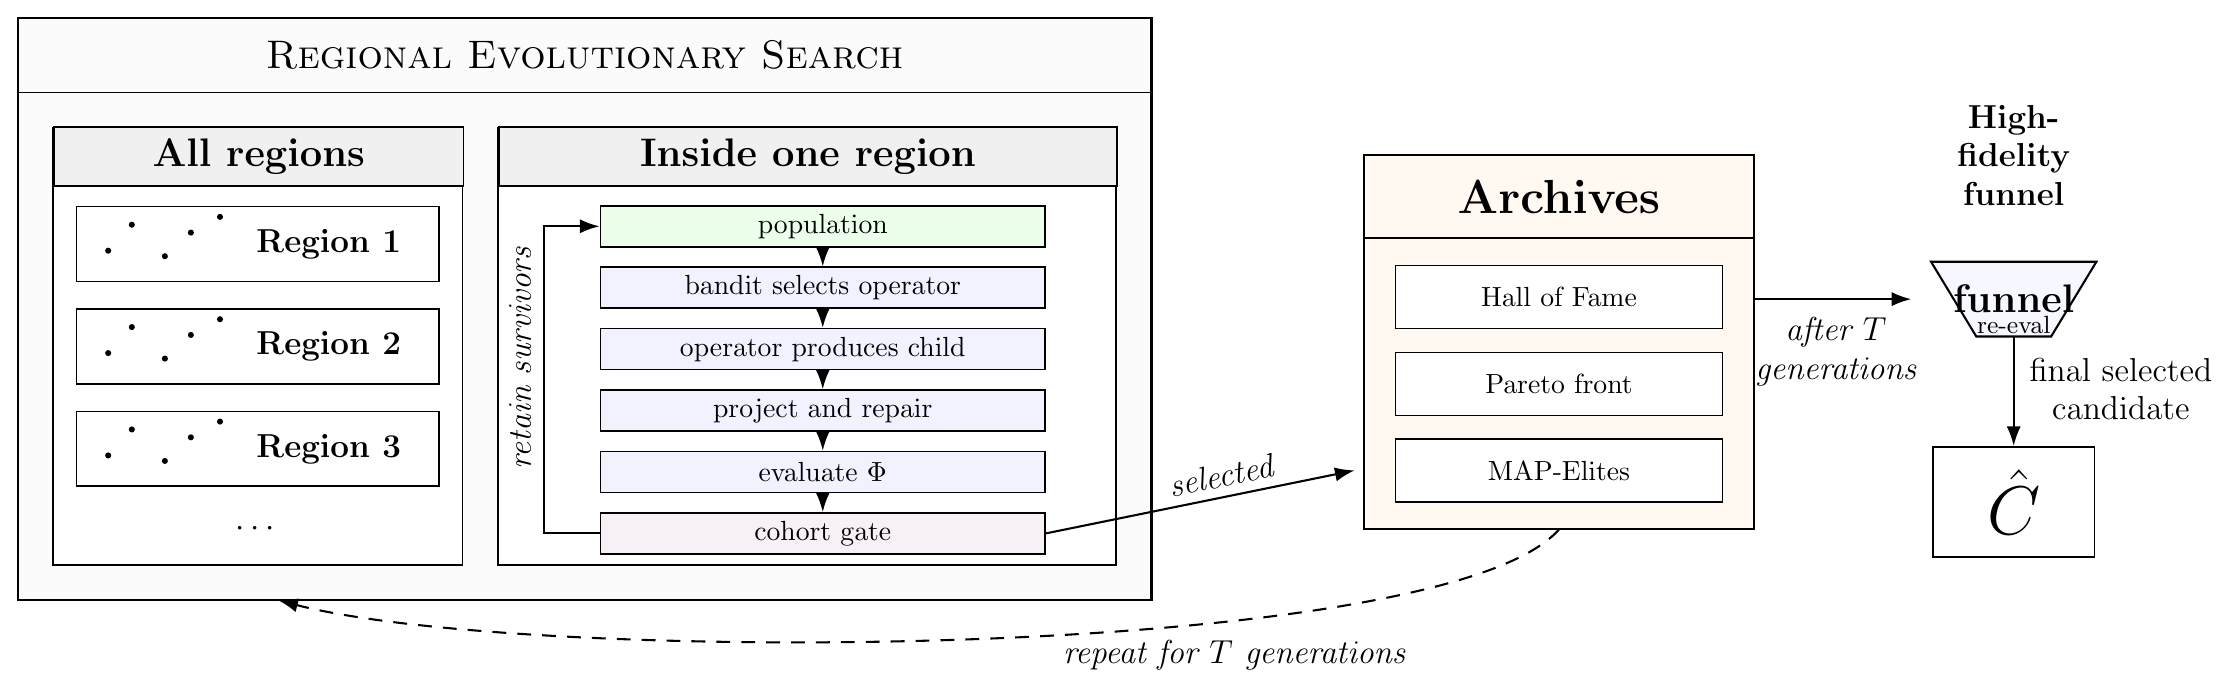
\includegraphics[width=0.95\linewidth]{figures/ga_overview_4.png}
\caption{One iteration of the search and the final funnel. Each region's population produces offspring with operators chosen by its bandit; offspring are projected back into the region, evaluated on the calibration packs, ranked by the cohort gate, and used to update the population and the archives. After $T$ iterations, the archives and the per-region best candidates are re-evaluated at higher fidelity and one mask $\widehat{\cand}$ is returned.}
\label{fig:ga_overview_4}
\end{figure}
